% !TEX root = SystemTemplate.tex

\chapter{Design  and Implementation}
This section is used to describe the design details for each of the major components in the system. The autonomous systems of teh UAV can be broken into individual components and the following sections will be divided by such. The first section will cover our simulation environment, the second will cover the autonomous takeoff and waypoint navigation, the third section will discuss our two autonomous landing approaches, and finally the fourth section will cover the UAV.      

\section{Simulation Environment}
\subsection{Technologies  Used}
The simulation environment will be implemented using Gazebo as the actual environment itself and will use ROS so we can use the message passing services to communicate with different modules of code that will be written. This environment will handle all testing so nothing is tested on the physical UAV until it is verified working in a simulated environment that utilizes a pixhawk.
\subsection{Component  Overview}
\begin{itemize}
  \item Ubuntu 14.04 LTS
  \item Gazebo
  \item Mavlink
  \item python
  \item c++
  \item R.O.S.
  \item Mavros (Ros wrapper around Mavlink)
\end{itemize}
\subsection{Phase Overview}
The simulation environment is still a work in progress on setting up communication with a simulated pixhawk with software in the loop (SITL), however as soon as the pixhawk is received hardware in the loop (HITL) will be attempted because of issues simulating the device. Issues as of now are loading a waypoint file and sending commands. A file checksum appears to be invalid for the waypoint file and a invalid flight controller unit is returned after sending commands to the simulated pixhawk with the mavros cmd node.
\subsection{Design Details}
Currently the Design for the simulation is relying on outside sources for installing the environment and setting up packages. These details are discussed in the Prototype section within sprint report \#3.


\section{Autonomous Takeoff and Waypoint Navigation} 
\subsection{Technologies  Used}
The autonomous takeoff and waypoint navigation system is separate from the simulation environment and landing approaches because these will be contained in a mission that will be uploaded into the pixhawk. There will be a waypoint publisher (wpt\_pub) node that will receive input from a user and create a mission file out of that input. Another module within the node will start publishing waypoints to the node so that it nodes what path to take what to do using mavros messages.
\subsection{Component  Overview}
wpt\_pub dependencies:
\begin{itemize}
  \item Ubuntu 14.04 LTS
  \item python
  \item c++
  \item R.O.S.
  \item Mavros
  \item Mavros msgs
\end{itemize}
\subsection{Phase Overview}
The wpt\_pub node can currently publish mavros messages that contain take off, land, and arm commands successfully, however the simulated pixhawk reports back that it is an invalid flight controller unit most times. It does receive waypoints successfully through mavros messages.
\subsection{Design Details}
\lstinputlisting[language=C++]{code/wpt_pub.hpp}
\lstinputlisting[language=C++]{code/wpt_pub.cpp}
\lstinputlisting[language=C++]{code/wpt_pub_node.cpp}

\newpage
\section{Landing Approaches}
\subsection{Visual Homography}
One of the approaches we will be using for the task of landing the UAV will be using visual homography. The basic goal here is to take an image that will contain the landing pad, and, based on the how the target looks on the pad, determine range to pad, orientation with respect to the pad, and the angle above the horizon with respect to the pad. This information will then be used to determine how to actually fly the UAV so that it will be able to safely land on the pad.
\subsubsection{Technologies  Used}
In order to accomplish this, we will use a number of tools. First and foremost, we will be using OpenCV as our image recognition library. OpenCV is a powerful open-source toolkit that will be able to handle any image processing that we need to do. The algorithm will be developed in Python, as this provides an easy-to-understand syntax, and will be able to deliver the performance that we need.
\subsubsection{Component  Overview}
\begin{itemize}
	\item Ubuntu 14.04 LTS
	\item Python
	\item OpenCV
\end{itemize}
\subsubsection{Phase Overview}
The algorithm is still a work in progress, but steps have been made. We have been able to compile and run last year's code, and have a working blob detection system up and running. This system is able to detect a pad with three colored circles by looking for the colors of the circles. The circles are red, green, and blue. It is then able to calculate the distance to the target, since it knows what size the target should be. This should be very helpful moving forward, as we are able to find the pad. In the coming sprints, we will attempt to move toward a pad that has four circles, as we believe this will give us more information to use for our homography computations.
\subsubsection{Design Details}
In the following image, you can see results from last year's code running and detecting the colored circles on a large target with three circles.

\begin{center} 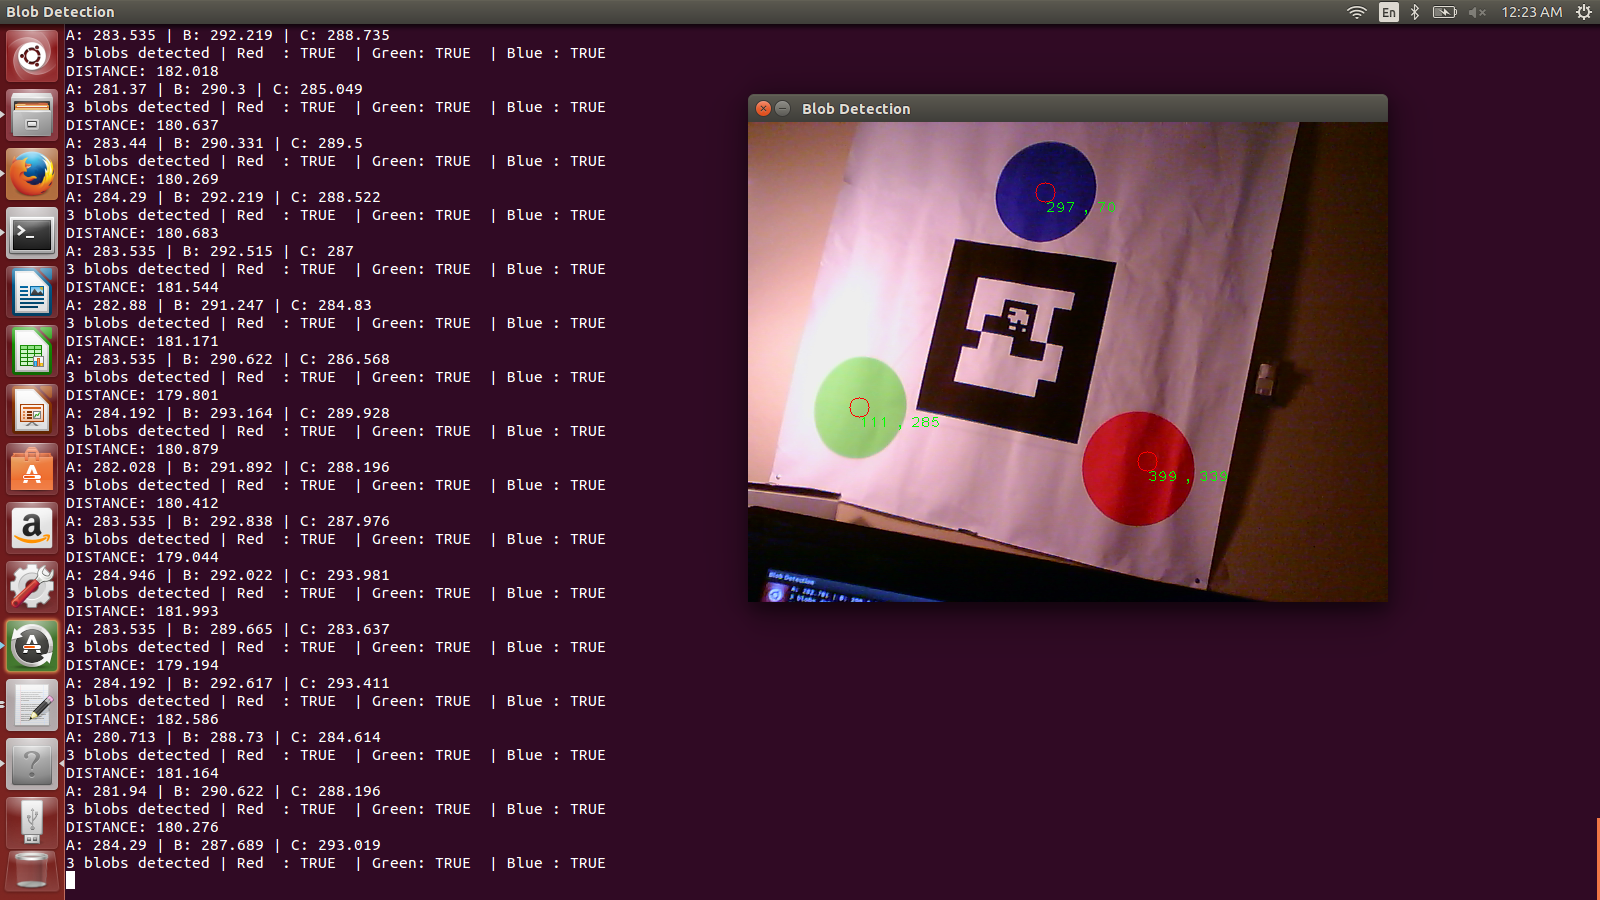
\includegraphics[width=.5\textwidth]{images/coolpic.png} \end{center}

It may be hard to notice, but the text that is currently being displayed in the terminal window shows that there are three blobs detected, exactly one for each color. It is also displaying the range to target, which is correct as far as we can tell.

The next image is what we are going to attempt to use for the next target. It has four colored circles, so we should be able to compute homography more accurately.

\begin{center} 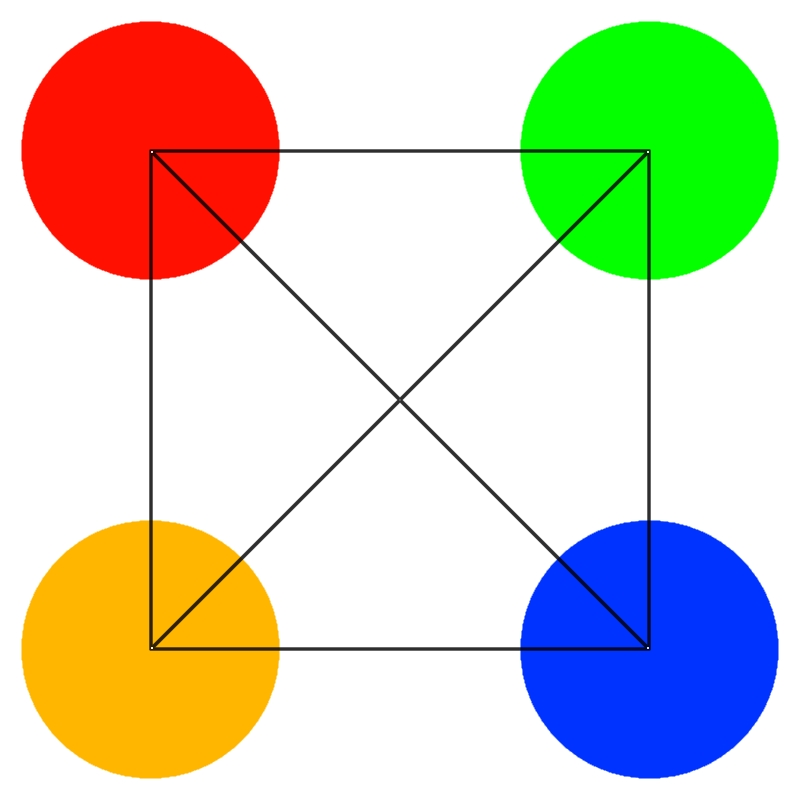
\includegraphics[width=.35\textwidth]{images/landing_guide_small_x.jpg} \end{center}

The final image is just another possible method that we have briefly explored where instead of blob detection we use hough transforms to detect only circles in the images. We have seen papers where others have had successes using targets consisting of concentric circles, so we think that we may be able to have some amount of success with this, in the event that the above methods don't end up panning out.

\begin{center} 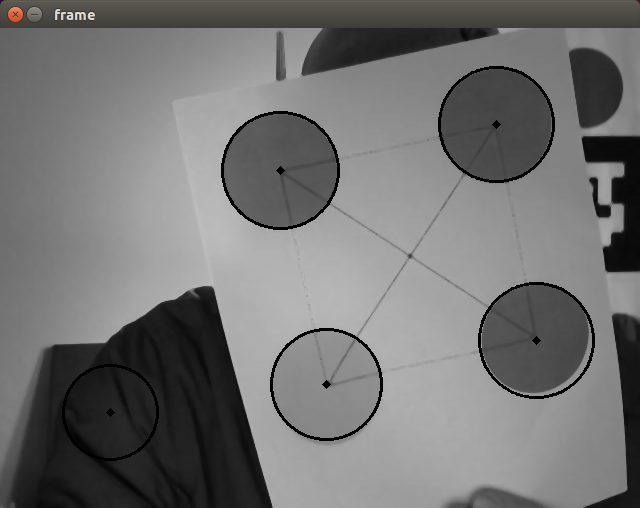
\includegraphics[width=.5\textwidth]{images/circles.png} \end{center}

\subsection{Reinforcement Learning}
\subsubsection{Technologies  Used}
To accomplish the reinforcement learning approach we will be using gazebo and ROS so that we can visually see that the agent is learning the states and actions required to land the UAV.  
\subsubsection{Component  Overview}
\begin{itemize}
  \item Ubuntu 14.04 LTS
  \item Python
  \item C++
  \item ROS pose messages
  \item sarsa\_alg: \\
  \\
  The class that instantiates the agent and performs the appropriate calculations to pick an action to move on to the next state and recieves a reward. Each action will send the appropriate messages to gazebo so that the UAV moves accordingly and allows the user to visually see what the agen is doing.
  \item sarsa\_node: \\
  \\
  The ROS nod that creates the sarsa\_alg class and handles initial topics to publish to and receive from.
\end{itemize}
\subsubsection{Phase Overview}
The Linear, gradient-descent Sarsa($lambda$) with binary features and $\epsilon$-greedy policy will be the algorithm of reinforcement learning that will be implemented. Currently ideas for using a 2-D state space are in the works with a vector field graient to be the actions to funnel the UAV into the center of a cone at a given height and radius. Because of the setbacks of the simulation no coding as been accomplished, but will be as soon as an environment is set up.

\subsubsection{Design Details}
\begin{algorithm} [h]                     % enter the algorithm environment
\caption{Linear, gradient-descent Sarsa($\lambda$) with binary features and $\epsilon$-greedy policy}         
 % give the algorithm a caption
\label{Sarsa}                           % and a label for \ref{} commands later in the document
\begin{algorithmic}                  % enter the algorithmic environment
    \STATE Initialize $\vec{\theta}$ arbitrily and $\vec{e} = \vec{0}$
    \FOR{Each Episode}
      \STATE $s \leftarrow$ initial state of episode
      \FOR{all $a \in A(s)$}
        \STATE $F_a \leftarrow$ set of features present in s, a
        \STATE $Q_a \leftarrow \sum_{i \in F_a}\theta(i)$
      \ENDFOR
      \STATE $a \leftarrow$ arg $max_a Q_a$
      \STATE With probability $\epsilon: a \leftarrow$ a random action $\in A(s)$
      \FOR{ Each Step of Episode}
        \STATE $\vec{e} \leftarrow \gamma \lambda \vec{e}$
        \FOR{ All $\bar{a} \neq a$}
          \FOR{All $i \in F_{\bar{a}}$}
            \STATE $e(i) \leftarrow 0 $
          \ENDFOR
        \ENDFOR
        \FOR{All $i \in F_a$}
          \STATE $e(i) \leftarrow 1 $
        \ENDFOR
        \STATE Take action $a$, observe reward, r, and next state, s'
        \STATE $\delta \leftarrow r - Q_a$
        \FOR{All $a \in A(s')$}
          \STATE $F_a \leftarrow$ set of features present in s', a
          \STATE $Q_a \leftarrow \sum_{i \in F_a}\theta(i)$
        \ENDFOR
        \STATE $a' \leftarrow$ arg $max_a Q_a$
        \STATE With probability $\epsilon:a' \leftarrow$ a random action $\in A(s)$
        \STATE $\delta \leftarrow \delta + \gamma Q_{a'}$
        \STATE $\vec{\theta} \leftarrow \vec{\theta} + \alpha \delta \vec{e}$
        \STATE $a \leftarrow a'$
      \ENDFOR
      \STATE until $s'$ is terminal
    \ENDFOR
\end{algorithmic}
\end{algorithm} 

\newpage
\section{UAV Build}
This section details the physical building of the UAV that will be used in autonomous landing.
\subsection{Technologies  Used}
The technologies that we currently have are listed below and include the controllers required for autonomous flight.
\begin{itemize}
	\item Turnigy Talong V1.0 Hexcopter
	\item 6x DC Motors
	\item 6x Electronic Speed Controllers
	\item 3DR Pixhawk
	\item Odroid-XU4
\end{itemize}
\subsection{Phase Overview}
We are currently in the first phase of UAV construction. In this phase we have completed the construction of the \textbf{Turnigy Talong V1.0 Hexcopter} frame, and mounting all of the DC motors and electronic speed controllers.
\subsection{Design Details}
Current documentation on the build progress made in Sprint 3 is shown below in our BuildProcess.pdf document.
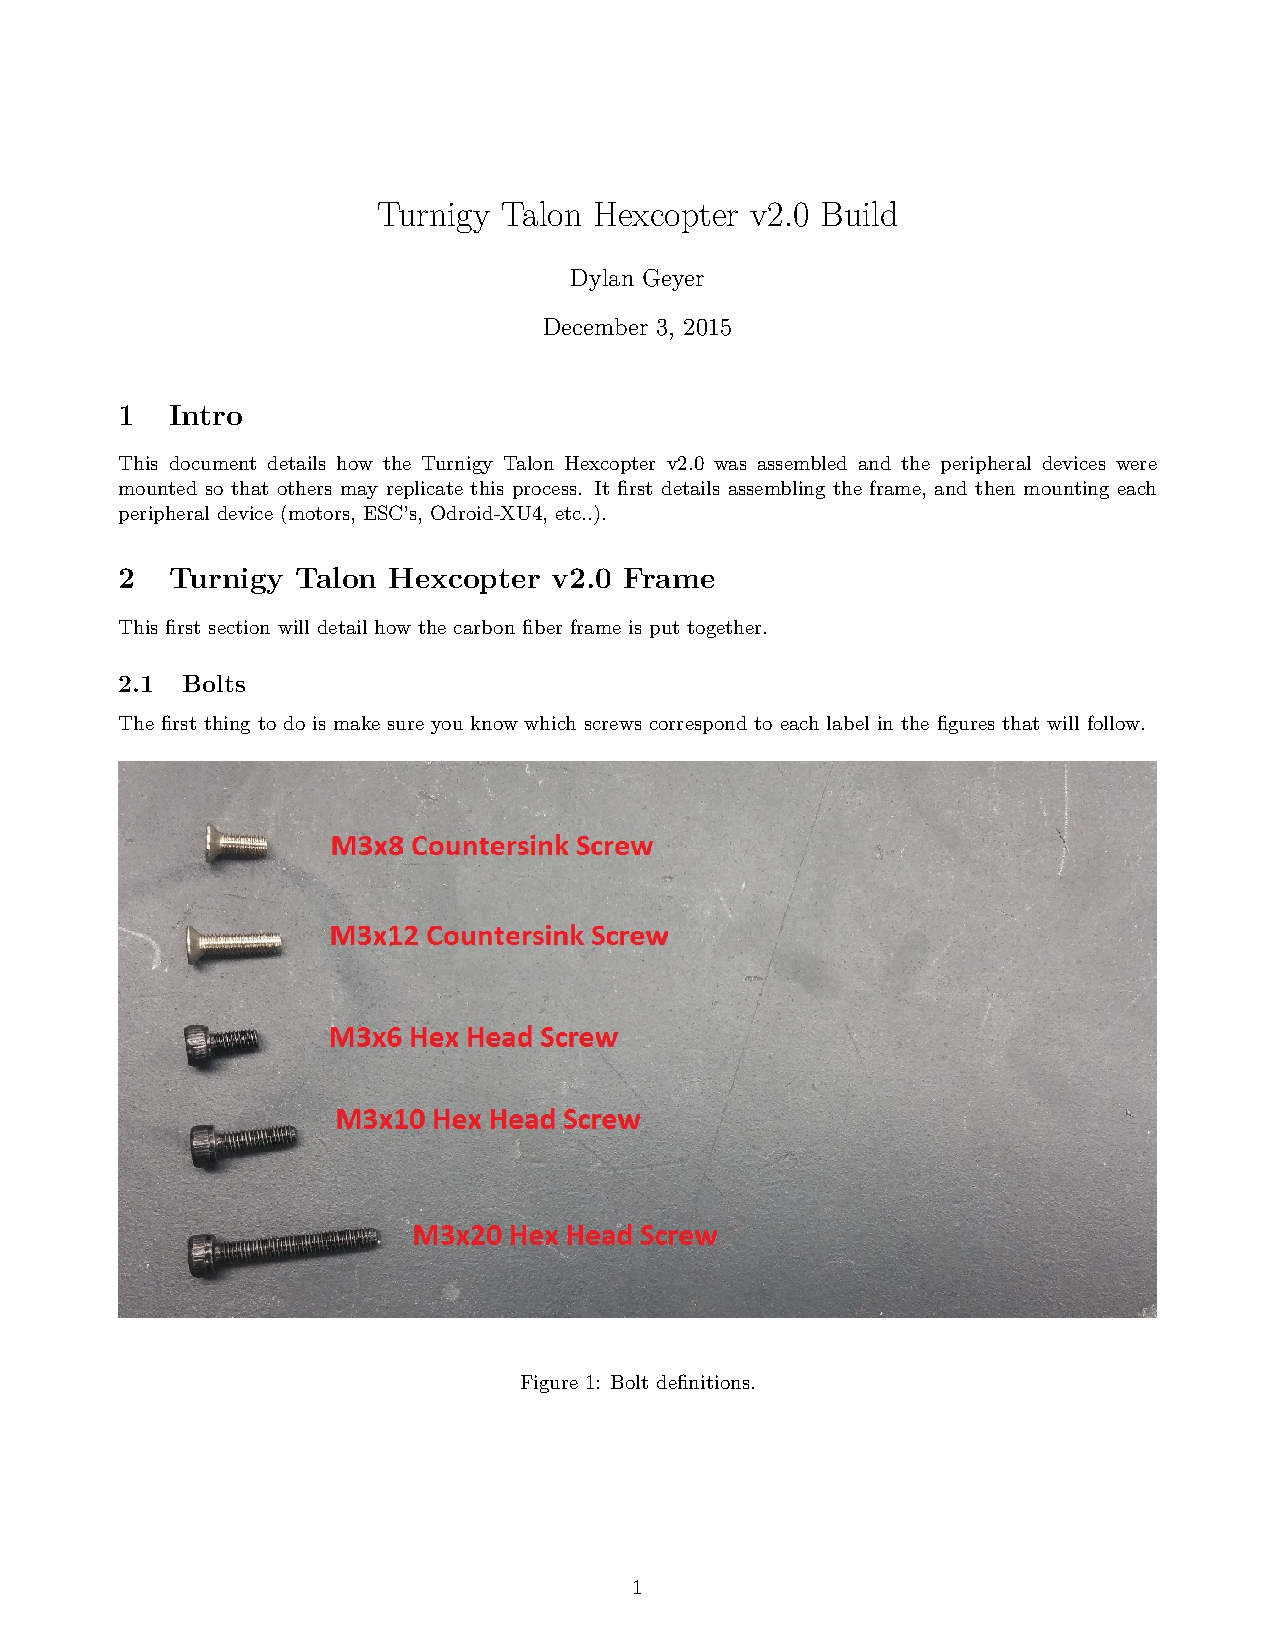
\includepdf[pages={1,2,3,4,5}]{../Documents/Prototypes/Sprint_3/BuildProcedure/BuildProcess.pdf}


%\begin{algorithm} [h]                     % enter the algorithm environment
%\caption{Calculate $y = x^n$}          % give the algorithm a caption
%\label{alg1}                           % and a label for \ref{} commands later in the document
%\begin{algorithmic}                    % enter the algorithmic environment
%    \REQUIRE $n \geq 0 \vee x \neq 0$
%    \ENSURE $y = x^n$
%    \STATE $y \Leftarrow 1$
%    \IF{$n < 0$}
%        \STATE $X \Leftarrow 1 / x$
%        \STATE $N \Leftarrow -n$
%    \ELSE
%        \STATE $X \Leftarrow x$
%        \STATE $N \Leftarrow n$
%    \ENDIF
%    \WHILE{$N \neq 0$}
%        \IF{$N$ is even}
%            \STATE $X \Leftarrow X \times X$
%            \STATE $N \Leftarrow N / 2$
%        \ELSE[$N$ is odd]
%            \STATE $y \Leftarrow y \times X$
%            \STATE $N \Leftarrow N - 1$
%        \ENDIF
%    \ENDWHILE
%\end{algorithmic}
%\end{algorithm} 
 
%\begin{lstlisting}
%#include <stdio.h>
%#define N 10
%/* Block
% * comment */
% 
%int main()
%{
%    int i;
% 
%    // Line comment.
%    puts("Hello world!");
% 
%    for (i = 0; i < N; i++)
%    {
%        puts("LaTeX is also great for programmers!");
%    }
% 
%    return 0;
%}
%\end{lstlisting}
%This code listing is not floating or automatically numbered.  If you want auto-numbering, but it in the algorithm environment (not algorithmic however) shown above.

\newpage
\section{Software: ROS Vision}
This section serves as an overview of the packages used to determine the landing pad, as well as estimate pose, by means of monocular vision. This description will include the packages, launch files, as well as other files needed to implement the AR tag tracking and pose estimation activities. This section is divided into sections covering the different portions of the ROS Vision build, as follows:
\begin{itemize}
\item Camera Operation
\item Camera Calibration
\item Image Processing
\item AR Tag Tracking
\item Pose Estimation
\end{itemize}

\subsection{Camera}
\textbf{usb\_cam}: this ros package provides a method for bringing usb cameras into the ros environment. The node will publish an image topic. 

\begin{itemize}
\item Parameters
\begin{itemize}
\item image width:
\item image height:
\item pixel\_format:
\item io\_method:
\item camera\_frame\_id:
\item framerate:
\item brightness:
\item saturation:
\item sharpness:
\item autofocus:
\item camera\_info\_url:
\item camera\_name:
\end{itemize}
\item Published Topics
\begin{itemize}
\item /image - containing the sensor\_msgs/Image message
\end{itemize}
\item installation: sudo apt-get-install ros-jade-usb-cam
\item Sample Launch File
\lstset{language=XML}
\begin{lstlisting}
<launch>
	<node pkg="usb_cam" type="usb_cam_node" name="usb_cam">
		<param name="video_device" type="string" value="/dev/video0"/>
		<param name="image_width" type="int" value="640" />
		<param name="image_height" type="int" value="480" />
		<param name="pixel_format" type="string" value="yuyv"/>
		<param name="camera_frame_id" value="camera" />
	</node>
</launch>
\end{lstlisting}
\end{itemize}



 
\noindent \textbf{pointgrey\_camera\_driver}: this ros package provides a method for bringing point grey cameras into the ros environment. 

\begin{itemize}
\item Parameters
\begin{itemize}
\item video\_mode:
\item frame\_rate:  the camera speed in frames per second
\item auto\_exposure:  Allow the camera to automatically change exposure (Combined Gain, Iris \& Shutter control).
\item exposure: 
\item auto\_shutter:
\item auto\_gain:
\item gain:
\item pan:
\item tilt:
\item brightness:
\item gamma:
\item auto\_white\_balance:
\item white\_balance\_blue:
\item white\_balance\_red:
\end{itemize}
\item Published Topics
\begin{itemize}
\item /image - containing the sensor\_msgs/Image message
\end{itemize}
\item installation: sudo apt-get install ros-jade-pointgrey-camera-driver
\item Usage:
\lstset{language=XML}
\begin{lstlisting}
<launch>
   <!-- Determine this using rosrun pointgrey_camera_driver list_cameras.
       If not specified, defaults to first camera found. -->
  <arg name="camera_serial" default="0" />
  <arg name="calibrated" default="0" />

  <group ns="camera">
    <node pkg="nodelet" type="nodelet" name="camera_nodelet_manager" 
     args="manager" />

    <node pkg="nodelet" type="nodelet" name="camera_nodelet"
          args="load pointgrey_camera_driver/PointGreyCameraNodelet 
                camera_nodelet_manager" >
      <param name="frame_id" value="camera" />
      <param name="serial" value="$(arg camera_serial)" />

      <!-- When unspecified, the driver will use the default framerate 
           as given by the camera itself. Use this parameter to override
           that value for cameras capable of other framerates. -->
      <!-- <param name="frame_rate" value="15" /> -->
      
      <!-- Use the camera_calibration package to create this file -->
      <param name="camera_info_url" if="$(arg calibrated)"
             value="file://$(env HOME)/.ros/camera_info/
                    $(arg camera_serial).yaml" />
    </node>

    <node pkg="nodelet" type="nodelet" name="image_proc_debayer"
          args="load image_proc/debayer camera_nodelet_manager">
    </node>
  </group>
</launch>
\end{lstlisting}
NOTE: This launch file is THE launch file provided by the repository, and will be available when you install this package. A few notes about what is occuring in this file before we go any further. The call for a camera calibration file will become clear in the next subsection. Additionally, this launch file is somewhat complicated by the use of nodelets which is a thing in ROS designed to reduce the complexity of the node networks in terms of communication. In the words of the ROS deities at \href{http://www.clearpathrobotics.com/guides/ros/Nodelet%20Everything.html}{Clear Path Robotics}
\begin{quotation}
The primary advantage is the automagic zero-copy transport between nodelets (in one nodelet manager). This means that the pointcloud created by a hardware driver doesn’t need to get copied or serialized before it hits your code, assuming you inject the nodelet into the camera’s manager, saving you time and trouble.

You get all the modularity of nodes, and all the efficiency of having one monolithic process. This makes nodelets more flexible than bare plugins (via pluginlib) - you can implicitly tap into any of the intra-process communication that occurs.
\end{quotation}
We leave it to the reader to learn more about nodelets should that be a path that appears to offer substantial benefit. The team made modifications to this file that will be discussed in a later subsection.
\end{itemize}

\subsection{Camera Calibration}
\noindent \textbf{camera\_calibration}: This package is used to calibrate both monocular and stereo cameras. The package has two functions, camera calibration and camera check. Camera check is to check the calibration of the camera. This may be a good idea to use after calibration is performed as an extra measure to ensure a good calibration was made by the calibration step. \par 

\noindent Before starting, it is necessary to get a calibration board. For this calibration, a chess board image is required. The interior corner count and size of chess board square in meters is needed.
\begin{itemize}
\item Subscribed Topics
\begin{itemize}
\item video\_mode:
\item frame\_rate:  the camera speed in frames per second
\item auto\_exposure:  Allow the camera to automatically change exposure (Combined Gain, Iris \& Shutter control).
\item exposure: 
\item auto\_shutter:
\item auto\_gain:
\item gain:
\item pan:
\item tilt:
\item brightness:
\item gamma:
\item auto\_white\_balance:
\item white\_balance\_blue:
\item white\_balance\_red:
\end{itemize}
\item installation: ssudo apt-get install ros-jade-camera-calibration
\item Usage:
\begin{enumerate}
\item start camera in ROS environment
\item begin camera calibration by using the following sample (\href{http://wiki.ros.org/camera_calibration}{found at the package documentation site}):
\begin{lstlisting}[language=bash]
$ rosrun camera_calibration cameracalibrator.py --size 8x6 --square 0.108 image:=/my_camera/image camera:=/my_camera
\end{lstlisting}
\end{enumerate}
\end{itemize}

\subsection{Image Processing}
\noindent \textbf{pointgrey\_camera\_driver}: this ros package provides a method for bringing point grey cameras into the ros environment. 

\begin{itemize}
\item Parameters
\begin{itemize}
\item video\_mode:
\item frame\_rate:  the camera speed in frames per second
\item auto\_exposure:  Allow the camera to automatically change exposure (Combined Gain, Iris \& Shutter control).
\item exposure: 
\item auto\_shutter:
\item auto\_gain:
\item gain:
\item pan:
\item tilt:
\item brightness:
\item gamma:
\item auto\_white\_balance:
\item white\_balance\_blue:
\item white\_balance\_red:
\end{itemize}
\item installation: sudo apt-get install ros-jade-pointgrey-camera-driver
\end{itemize}

\subsection{Tag Tracking}
\noindent \textbf{pointgrey\_camera\_driver}: this ros package provides a method for bringing point grey cameras into the ros environment. 

\begin{itemize}
\item Parameters
\begin{itemize}
\item video\_mode:
\item frame\_rate:  the camera speed in frames per second
\item auto\_exposure:  Allow the camera to automatically change exposure (Combined Gain, Iris \& Shutter control).
\item exposure: 
\item auto\_shutter:
\item auto\_gain:
\item gain:
\item pan:
\item tilt:
\item brightness:
\item gamma:
\item auto\_white\_balance:
\item white\_balance\_blue:
\item white\_balance\_red:
\end{itemize}
\item installation: sudo apt-get install ros-jade-pointgrey-camera-driver
\end{itemize}

\subsection{Localization}
\noindent \textbf{pointgrey\_camera\_driver}: this ros package provides a method for bringing point grey cameras into the ros environment. 

\begin{itemize}
\item Parameters
\begin{itemize}
\item video\_mode:
\item frame\_rate:  the camera speed in frames per second
\item auto\_exposure:  Allow the camera to automatically change exposure (Combined Gain, Iris \& Shutter control).
\item exposure: 
\item auto\_shutter:
\item auto\_gain:
\item gain:
\item pan:
\item tilt:
\item brightness:
\item gamma:
\item auto\_white\_balance:
\item white\_balance\_blue:
\item white\_balance\_red:
\end{itemize}
\item installation: sudo apt-get install ros-jade-pointgrey-camera-driver
\end{itemize}
